\documentclass{report}
\usepackage{algorithmicx, algpseudocode, graphicx}

\begin{document}
\title{CHEERS}
\author{Team E}
\date{22 Feb 2023}
\maketitle

\chapter*{CRC Cards}
\begin{figure}[h!]
    \centering
    \begin{tabular}{@{}c@{}}
      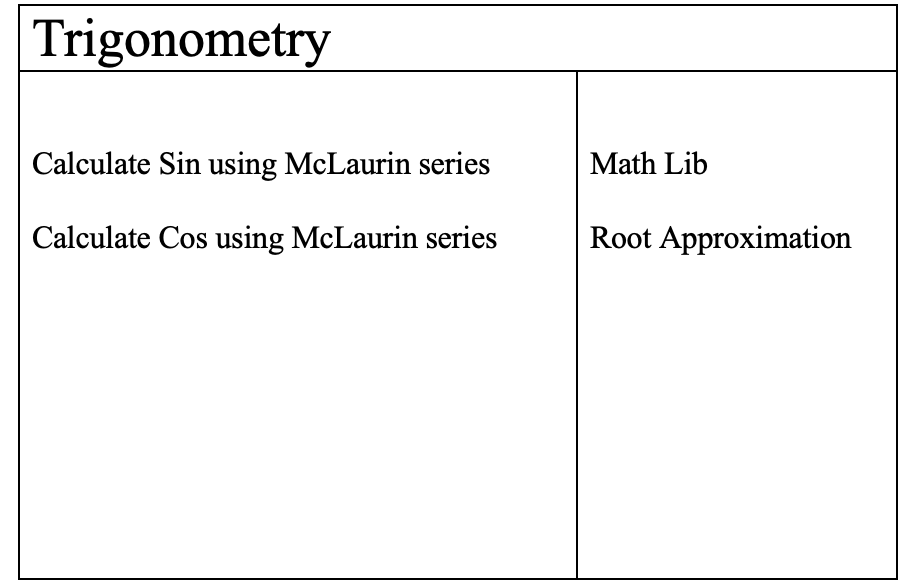
\includegraphics[width=.4\linewidth]{resources/Trigonometry.png} 
        \hspace*{30pt}
      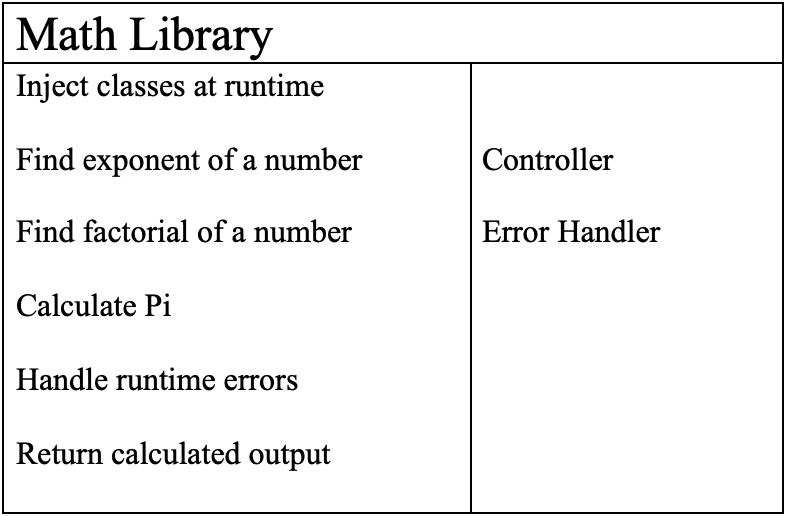
\includegraphics[width=.4\linewidth]{resources/MathLib.png}
    \end{tabular}
  
    \begin{tabular}{@{}c@{}}
        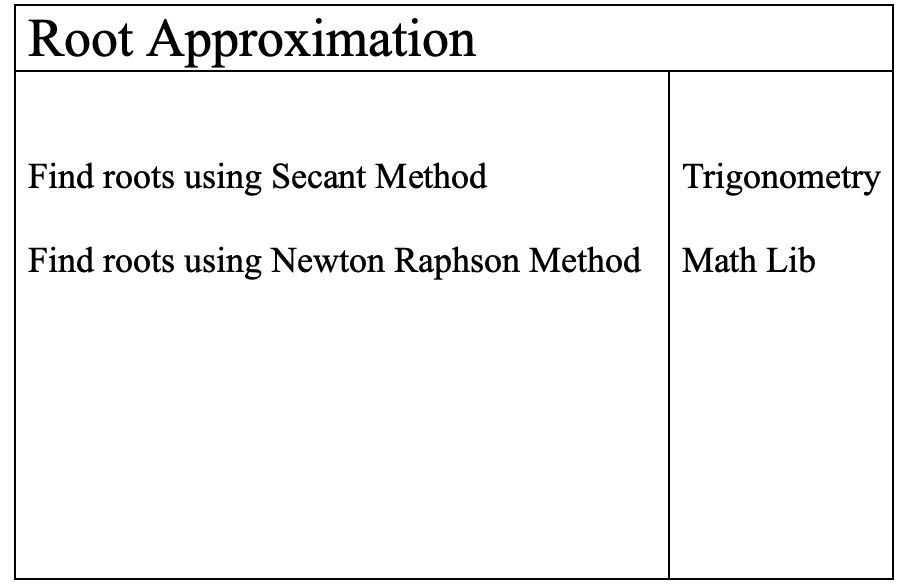
\includegraphics[width=.4\linewidth]{resources/RootApproximation.png} 
          \hspace*{30pt}
        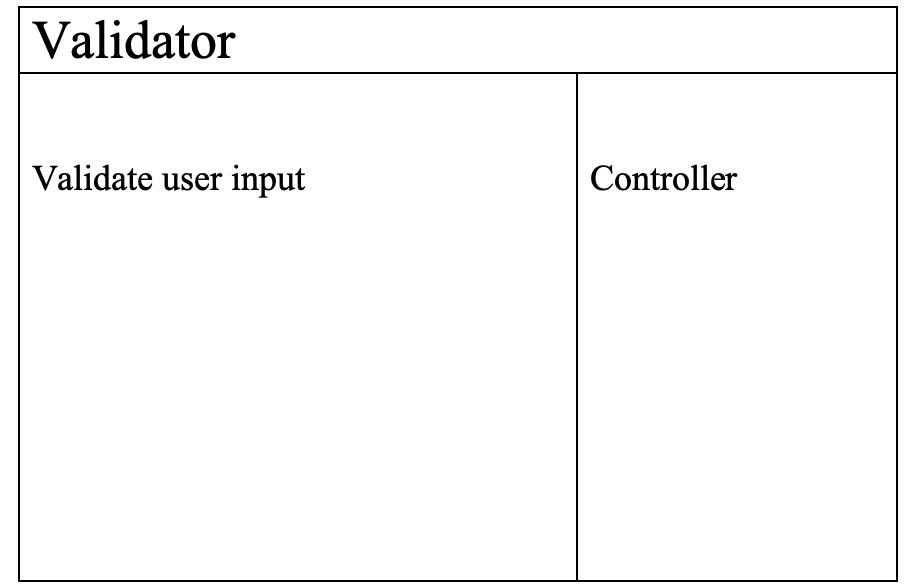
\includegraphics[width=.4\linewidth]{resources/Validator.png}
      \end{tabular}

      \begin{tabular}{@{}c@{}}
        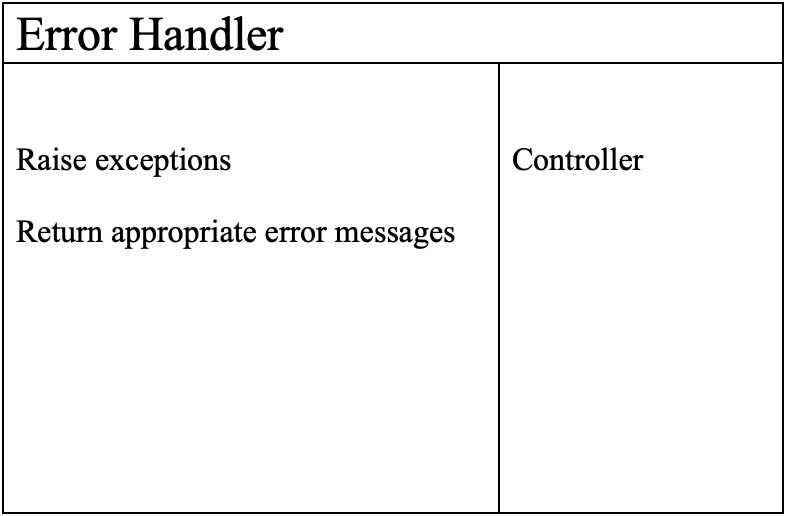
\includegraphics[width=.4\linewidth]{resources/ErrorHandler.png} 
          \hspace*{30pt}
        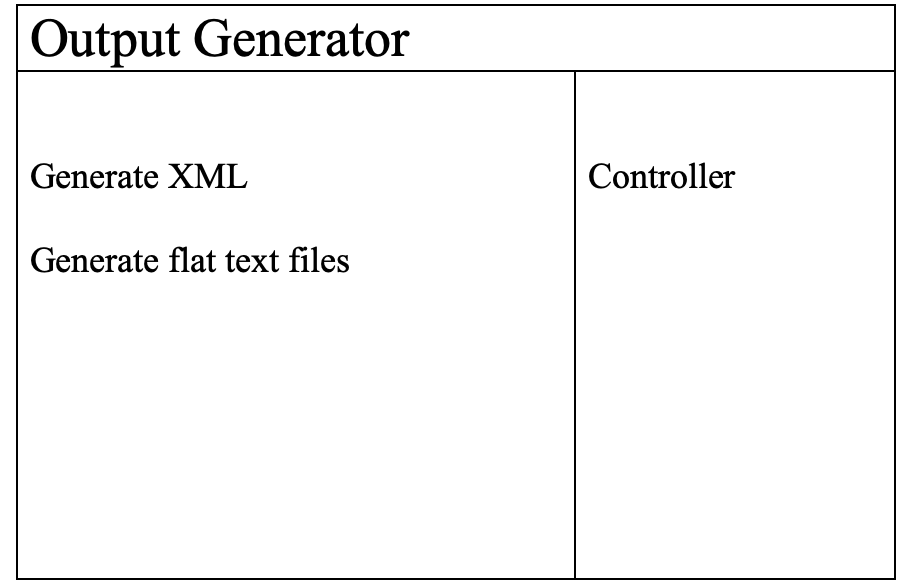
\includegraphics[width=.4\linewidth]{resources/OutputGenerator.png}
      \end{tabular}
      
      \begin{tabular}{@{}c@{}}
        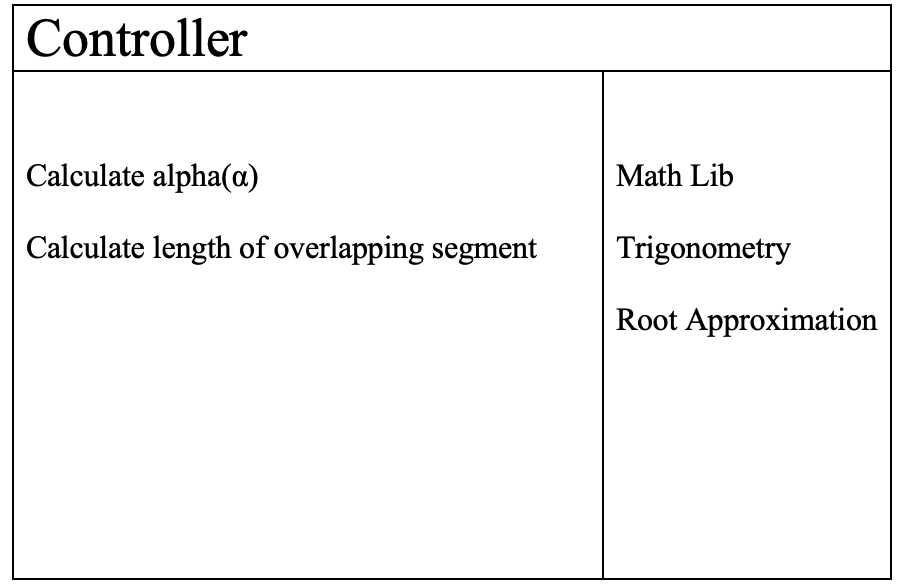
\includegraphics[width=.5\linewidth,height=90pt]{resources/Controller.png}
      \end{tabular}

      \vspace{\floatsep}
    \caption{CRC Cards for CHEERS}\label{fig:myfig}
\end{figure}

\chapter*{Pseudocode}
\section{Sin using Mclaurin}
We arrive at a value for sin of a number using the Mclaurin series expansion.
\break
\begin{algorithmic}[1]
    \Function{calculate\_sin}{$rad$}
        \State $total\_iterations \gets precision$
        \State $sin\_val \gets 0$
        \For{$i \gets 0, total\_iterations$}
            \State $term \gets (-1)^i \cdot rad^{2i + 1} / (2i + 1)!$
            \State $sin\_val \gets sin\_val + term$
        \EndFor
        \State \Return $sin\_val$
    \EndFunction
\end{algorithmic}

\section{Secant Approximation}
The roots of an equation can be derived using the secant approximation method.
\break
\begin{algorithmic}[1]
\Function{secant\_approximation}{func, $x_0$, $x_1$, $e$}
    \State $x_2 \gets 0$
    \State $step \gets 1$
    \While{True}
        \If{func($x_0$) == func($x_1$)}
            \State \textbf{break}
        \EndIf
        \State $x_2 \gets x_0 - (x_1 - x_0) * func(x_0) / (func(x_1) - func(x_0))$
        \State $x_0 \gets x_1$
        \State $x_1 \gets x_2$
        \State $step \gets step + 1$
        \If{$step > num\_terms$}
            \State \textbf{print}("Not convergent")
            \State \textbf{break}
        \EndIf
        \If{func($x_2$) - func($x_1$) $>$ e}
            \State \textbf{break}
        \EndIf
    \EndWhile
    \State \textbf{return} $x_2$
\EndFunction
\end{algorithmic}

\section{Pi Calculation}
The algorithm to calculate the value of Pi is the following.
\break
\begin{algorithmic}[1]
    \Function{CalculatePi}{}
        \State $val \gets 0.0$
        \State $total\_terms \gets 100$
        \For{$i=1$ to $2*total\_terms$}
            \State $sign \gets -(i\%4-2)$
            \State $val \gets val + \frac{sign}{i}$
        \EndFor
        \State \Return $4 * val$
    \EndFunction
\end{algorithmic}

\section{Exponent}
The exponent of a number can be obtained using the following algorithm.
\break
\begin{algorithmic}[1]
\Function{exp}{$number$, $power$}
    \If{$power = 0$}
        \State \Return $1$
    \EndIf
    \State $temp \gets$ \Call{exp}{$number$, $\lfloor power/2 \rfloor$}
    \If{$power$ is even}
        \State \Return $temp * temp$
    \Else
        \State \Return $temp * temp * number$
    \EndIf
\EndFunction
\end{algorithmic}

\section{Factorial}
This is the algorithm used to obtain the factorial of a number.
\break
\begin{algorithmic}[1]
\Function{factorial}{$num$}
  \If{$num < 0$}
    \State \textbf{raise} Exception(``Factorial can't be calculated for negative numbers'')
  \EndIf
  \State $result \gets 1$
  \For{$i \gets 1$ \textbf{to} $num$}
    \State $result \gets result \times i$
  \EndFor
  \State \textbf{return} $result$
\EndFunction
\end{algorithmic}


\end{document}